%auto-ignore
\providecommand{\MainFolder}{..}
\documentclass[\MainFolder/Text.tex]{subfiles}

\begin{document}

\section{Construction of a Hodge propagator for spheres}
\label{Sec:GreenSphere}

The standard Riemannian volume form on the round sphere $\Sph{n}\subset \R^{n+1}$ is the restriction of the following closed form on $\R^{n+1}\backslash \{0\}$:  
$$ \Vol(x) \coloneqq \frac{1}{|x|^{n+1}}\sum_{i=1}^{n+1} (-1)^{i+1} x^i \Diff x_1 \dotsm \widehat{\Diff x_i} \dotsm \Diff x_{n+1}. $$
Here $\widehat{\Diff x_i}$ means that $\Diff{x_i}$ is omitted. We denote the Riemannian volume of $\Sph{n}$ by
$$ V\coloneqq \int_{\Sph{n}} \Vol. $$
The $n$-form $\HKer$ from Proposition~\ref{Lemma:HKer} reads
\begin{equation*}
\HKer =  \frac{1}{V}\bigl(\Pr_1^*\Vol +  (-1)^{n} \Pr_2^*\Vol\bigr).
\end{equation*}
According to Proposition~\ref{Prop:GKer}, the equation which we want to solve reads
\begin{equation} \label{Eq:GreenKernel}
\Dd \Prpg = \frac{1}{V}\bigl((-1)^{n}\Pr_1^*\Vol +  \Pr_2^*\Vol\bigr).
\end{equation}
We denote 
$$\tilde{G}\coloneqq V\Prpg\quad\text{and}\quad \tilde{H}\coloneqq V\HKer.$$

The following lemma will be used to construct a solution to~\eqref{Eq:GreenKernel}. 
\begin{Lem}[Relative Poincar\'e Lemma]\label{Lem:ChainHtpy}
Let $M$ be a smooth oriented manifold and $\psi: [0,1]\times M \rightarrow M$ a smooth map. Consider the operator $T: \DR^*(M) \rightarrow \DR^{*-1}(M)$ defined by
$$ T(\eta) \coloneqq \FInt{[0,1]} \psi^*\eta\quad\text{for all }\eta\in \DR(M), $$
where we integrate along the fiber of the oriented fiber bundle $\Pr_2: [0,1]\times M \rightarrow M$. Then we have
$$ \Dd\circ T + T\circ \Dd = \psi_1^* - \psi_0^*. $$
\end{Lem}
%
\begin{proof}
Stokes' formula from Proposition~\ref{Prop:StokesForm} gives
$$ \Dd \FInt{[0,1]}\psi^*\eta = -\Bigl( \FInt{[0,1]} \Dd \psi^* \eta - \FInt{\Bdd [0,1]} \psi^* \eta \Bigr) = - \FInt{[0,1]} \psi^* \Dd \eta + \psi^*_1 \eta - \psi^*_0 \eta$$
for all $\eta \in \DR(M)$.
\end{proof}


\begin{Proposition}[Solution to \eqref{Eq:GreenKernel}] \label{Prop:GKerSph}
For all $(x,y)\in (\Sph{n}\times \Sph{n}) \backslash \Diag$, let
\begin{equation} \label{Eq:GreenKernelMC1}
\Prpg (x,y) \coloneqq (-1)^{n} \sum_{k=0}^{n-1} g_k(x,y)\omega_k(x,y),
\end{equation}
where
\begin{equation}\label{Eq:FunctionsGk1}
 g_k(x,y) \coloneqq \int_{0}^1 \frac{t^k(t-1)^{n-1-k}}{(2t(t-1)(1+x\cdot y) + 1)^{\frac{n+1}{2}}} \Diff{t}
\end{equation}
and 
\begin{equation} \label{Eq:FormOmega1}
\omega_k(x,y) \coloneqq \begin{multlined}[t]\frac{1}{k!} \frac{1}{(n-1-k)!} \sum_{\sigma \in \Perm_{n+1}} (-1)^\sigma x^{\sigma_1} y^{\sigma_2} \Diff{x^{\sigma_3}} \dotsm \Diff{x^{\sigma_{2+k}}} \\ \Diff{y^{\sigma_{3+k}}} \dotsm \Diff{y^{\sigma_{n+1}}}.\end{multlined}
\end{equation}
The form~\eqref{Eq:GreenKernelMC1} is a smoooth solution to~\eqref{Eq:GreenKernel} on $(\Sph{n}\times \Sph{n}) \backslash \Diag$.
\end{Proposition}
%\Red{Can $\omega$ be written as a product in the sense that in $n=1$ is $\omega_{00}=x\cdot Ry$.?}
%
\begin{proof} %Checked on 19.9.17 
Define the set
$$ N \coloneqq (\R^{n+1}_{\neq 0}\times\R^{n+1}_{\neq 0})\backslash \{(x,a x) \mid x\in \R^{n+1}, a>0\}. $$
It is an open thickening of $(\Sph{n}\times \Sph{n})\backslash \Diag$ in $\R^{n+1} \times \R^{n+1}\backslash \Diag $. Consider the smooth deformation retraction
\begin{align*}
 \psi : [0,1] \times N & \longrightarrow N \\
 (t,x,y) &\longmapsto \psi_t(x,y) \coloneqq (x,(1-t)y-tx)
\end{align*}
with 
$$ \psi_0(x,y)=(x,y) \quad \text{and}\quad \psi_1(x,y)= (x,-x)\quad\text{for all }(x,y)\in N. $$
The retraction is depicted in Figure~\ref{Fig:Retraction}.
\begin{figure}
\centering
%\includegraphics[width=.3\textwidth,trim=5.1cm 20.5cm 7.6cm 1.3cm,clip]
%auto-ignore
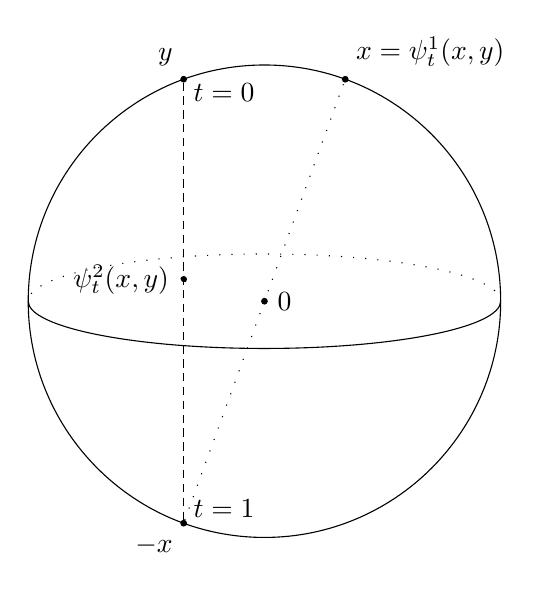
\begin{tikzpicture}
  \tikzset{point/.style = {draw, circle, fill=black, minimum size=2pt,inner sep=0pt}}
  \tikzset{->-/.style={decoration={markings,mark=at position #1 with {\arrow{>}}},postaction={decorate}}}
  \tikzset{-<-/.style={decoration={markings,mark=at position #1 with {\arrow{<}}},postaction={decorate}}}

  \def\rad{3cm}
  \def\posx{70}
  \def\posy{110}
  
  % Sphere
  \node [point,label={0:0}] (C) at (0,0) {};
  \draw (C) circle (\rad);
  \draw (-\rad,0) arc (180:360:3 and 0.6);
  \draw[loosely dotted] (\rad,0) arc (0:180:3 and 0.6);
  
  
  \path (C) node[point,label={\posx:$x=\psi^{1}_t(x,y)$}] (x)  at +(\posx:\rad) {};
  \path (C) node[point,label={\posx+180:$-x$}] (mx)  at +(\posx+180:\rad) {};
  \path (C) node[point,label={\posy:$y$}] (y)  at +(\posy:\rad) {};
  
  \draw[loosely dotted] (mx) -- (x);
  \draw[densely dashed] (y) node [label={[label distance=-6pt,yshift=1pt,xshift=1pt]-50:$t=0$}] {} -- node[point,pos=0.45,label={[left,label distance=-3pt]0:$\psi_t^{2}(x,y)$}] {} (mx) node [label={[label distance=-6pt,yshift=11pt,xshift=1pt]-50:$t=1$}] {};
\end{tikzpicture}
\caption[Retraction of the configuration space $C_2(\Sph{n})$ to $\Sph{n}$.]{Retraction $\psi_t = (\psi_t^1, \psi_t^2)$. A point of $\Sph{n}\times \Sph{n}$ is visualized as a pair of points on $\Sph{n}$.}\label{Fig:Retraction}
\end{figure}
Denote by $A: \R^{n+1} \rightarrow \R^{n+1}$, $x\mapsto -x$ the antipodal map. It is easy to see that 
$$ A^* \Vol = (-1)^{n+1} \Vol, $$
and hence
\begin{equation*}
\psi_1^* \tilde{\HKer} = \psi_1^* \Pr_1^*\Vol + (-1)^n \psi_1^*\Pr_2^* \Vol  = \Pr_1^*\Vol + (-1)^n \Pr_1^*A^* \Vol = 0. 
\end{equation*}
Define 
\begin{equation}  \label{Eq:GExpr}
\Prpg \coloneqq (-1)^{n+1} \FInt{[0,1]} \psi^*\HKer.
\end{equation}
Let $T: \DR^*(N)\rightarrow \DR^{*-1}(N)$ be the cochain homotopy from Lemma~\ref{Lem:ChainHtpy} associated to $\psi$. Because $\Dd \HKer=0$, we get
$$ \Dd \Prpg = (-1)^{n+1} \Dd T(\HKer) = (-1)^{n+1}(\Dd T + T \Dd)\HKer = (-1)^{n+1}(\psi_1^*-\psi_0^*)\HKer = (-1)^{n}\HKer. $$
For every $i=1$,~$\dotsc$, $n+1$, we have
$$ \psi^*(\Diff{x^i}) = \Diff{x^i}\quad\text{and}\quad\psi^*(\Diff{y^i}) = (1-t)\Diff{y^i} - t\Diff{x^i} - (y^i+x^i)\Diff{t}. $$
We compute
%
\begin{equation*}
\begin{aligned}
 & (-1)^{n+1} \FInt{[0,1]} \psi^* \tilde{\HKer} = -\FInt{[0,1]} \psi^* \Pr_2^* \Vol \\
 & \quad = \FInt{[0,1]} \sum_{i=1}^{n+1} (-1)^{i}\frac{((1-t)y^i - t x^i)}{{\Abs{(1-t)y-tx}^{n+1}}} \psi^*(\Diff{y^1} \dotsm \widehat{\Diff{y^i}} \dotsm \Diff{y^{n+1}}) \\
 & \quad = \sum_{1\le i<j \le n+1} (-1)^{i+j}(x^i y^j - y^i x^j) \FInt{[0,1]}  \frac{\Diff{t} \psi^*(\Diff{y^1} \dotsm \widehat{\Diff{y^i}} \dotsm \widehat{\Diff{y^j}} \dotsm \Diff{y^{n+1}})}{\Abs{(1-t)y-tx}^{n+1}} \\ 
 & \quad = \begin{multlined}[t] (-1)^{n}\sum_{k=0}^{n-1} \Bigl(\int_0^1 \frac{t^k(t-1)^{n-1-k}}{\Abs{(1-t)y-tx}^{n+1}} \Diff{t}\Bigr) \sum_{1\le i<j\le n+1} (-1)^{i+j+1} (x^i y^j - y^i x^j) \\
 \sum_{\mathclap{\substack{\sigma: \{1,\dotsc,n-1\}\rightarrow \{1,\dotsc,\hat{i},\dotsc,\hat{j},\dotsc,n+1\} \\ \sigma_1<\dots < \sigma_k \\ \sigma_{k+1}<\dots < \sigma_{n-1}}}} (-1)^\sigma \Diff{x^{\sigma_1}} \dotsm \Diff{x^{\sigma_k}}\Diff{y^{\sigma_{k+1}}} \dotsm \Diff{y^{\sigma_{n-1}}}.\end{multlined}
\end{aligned}
\end{equation*}
The formulas~\eqref{Eq:FunctionsGk1} and~\eqref{Eq:FormOmega1} are obtained from this by writing 
$$ \Abs{(1-t)y - tx}^2 = 2t(t-1)(1+x \cdot y) + 1 $$
in the denominator of the integrand and by simple combinatorics in the form part, respectively. Smoothness of~$\Prpg$ on $(\Sph{n}\times \Sph{n})\backslash \Diag$ follows from the expression~\eqref{Eq:GExpr}.
\end{proof}
Note that $g_k$ are smooth functions on $(\Sph{n}\times \Sph{n})\backslash \Diag$.
%
\begin{Example}[ for $\Sph{1}$ and $\Sph{2}$]\phantomsection\label{Example:Circle}% On 15.9.17
\begin{ExampleList}
\item Let 
$$\alpha: (\Sph{1}\times\Sph{1})\backslash \Diag \rightarrow (0,2\pi)$$
be the smooth function assigning to a pair $(x,y)\in  (\Sph{1}\times\Sph{1})\backslash \Diag$ the counterclockwise angle from $x$ to $y$. Let $\alpha_1$, $\alpha_2 \in [0,2\pi)$ be such that $x=\cos(\alpha_1)\StdBasis_1 + \sin(\alpha_1)\StdBasis_2$ and $y=\cos(\alpha_2)\StdBasis_1+\sin(\alpha_2)\StdBasis_2$ for the standard Euclidean basis $\StdBasis_1$, $\StdBasis_2$ of $\R^2$. It is easy to see that
$$ \alpha(x,y) = \begin{cases} \alpha_2 - \alpha_1 & \text{if }\alpha_1<\alpha_2, \\
\alpha_2-\alpha_1+2\pi & \text{if }\alpha_1>\alpha_2. \end{cases} $$
Therefore, we get
$$ \Diff{\alpha} = \Diff{\alpha_2} -\Diff{\alpha_1} = -2\pi H \quad\text{on } (\Sph{1}\times\Sph{1})\backslash \Diag. $$
On the other hand, we can compute $\Prpg$ from~\eqref{Eq:GreenKernelMC1} as follows. Using the substitution $u=2t-1$, we get for all $x$, $y\in \Sph{1}$ with $x\neq \pm y$ the following:
%
\begin{equation*}
\begin{aligned}
 g_{0}(x,y) &= \int_0^1 \frac{\Diff{t}}{2t(t-1)(1+x\cdot y) +1} =  \frac{1}{1-x\cdot y}\int_{-1}^1 \frac{\Diff{u}}{\frac{1+x\cdot y}{1- x\cdot y}u^2 + 1} \\ &= \frac{2}{\sqrt{1-(x\cdot y)^2}}\arctan\Bigl(\sqrt{\frac{1+x\cdot y}{1-x\cdot y}}\Bigr) \\ &= \frac{\pi - \arccos(x\cdot y)}{\sqrt{1-(x\cdot y)^2}}  = \frac{\pi - \arccos(x\cdot y)}{ \Abs{x^1 y^2 - x^2 y^1}} = \frac{\pi - \alpha(x,y)}{x^1 y^2 - x^2 y^1}.
\end{aligned}
\end{equation*}
The third from last equality can be obtained by trigonometric considerations and the second from last equality by an algebraic manipulation with the denominator. We will explain the last equality. Consider the matrix 
$$ R=\begin{pmatrix}
0 & -1 \\ 1 & 0
\end{pmatrix} $$
representing the counterclockwise rotation by $\frac{\pi}{2}$. The function $\arccos: (-1,1) \rightarrow (0,\pi)$ satisfies
$$ \arccos(x\cdot y) = \begin{cases}
                        \alpha(x,y) & \text{if }y\cdot Rx > 0, \\
                        2\pi - \alpha(x,y) & \text{if }y\cdot Rx<0. 
                       \end{cases}$$
The last equality becomes clear when we notice that $x^1 y^2 - x^2 y^1 = y\cdot Rx$. 

Finally, we have $\omega_{0}(x,y) = x^1 y^2 - x^2 y^1$, and hence
$$ 2\pi G(x,y) =  - g_{0}(x,y) \omega_{0}(x,y) = \alpha(x,y) - \pi = \pi - \alpha(y,x). $$
\item For $n=2$, we get the formulas
\allowdisplaybreaks
\begin{align*}
g_0(x,y) & = - g_1(x,y) = \frac{1}{x\cdot y - 1}\quad\text{and} \\
\omega_0(x,y) &=(x^2 y^3 - x^3 y^2) \Diff{y^1} +(x^3 y^1 - x^1 y^3) \Diff{y^2} + (x^1 y^2 - x^2 y^1) \Diff{y^3} \\ &=\sum_{i=1}^3 (x\times y)^i \Diff{y^i}.
\end{align*}
The formula for $\omega_1(x,y)$ is obtained from the formula for $\omega_0(x,y)$ by replacing~$\Diff{y}$ with $\Diff{x}$.\qedhere
\end{ExampleList}
\end{Example}

Consider the diagonal action of the orthogonal group $O(n+1)$ on $\R^{n+1}\times\R^{n+1}$ by matrix multiplication.
%$$ R(x,y)\coloneqq (Rx,Ry)\quad \text{for all }(x,y)\in \R^{n+1}\times\R^{n+1}, R\in O(n+1), $$ 
%where $Rx$ denotes the standard action on $\R^{n+1}$.
\begin{Proposition}[Symmetries of $\Prpg$]\label{Prop:SymmetryOfG}
Consider $\Prpg$ from Proposition~\ref{Prop:GKerSph}. For all $R\in O(n+1)$, we have
$$ R^* \Prpg = (-1)^R \Prpg, $$
where $(-1)^R = \det(R)$. Moreover, if $\tau$ denotes the twist map, then
$$\tau^*\Prpg = (-1)^{n}\Prpg. $$ 
\end{Proposition}
%
\begin{proof} % Check on 13.9.17
We will use the thickening $N$, the antipodal map $A$ and the expression~\eqref{Eq:GExpr} for~$\Prpg$ from the proof of Proposition~\ref{Prop:GKerSph}.

It is easy to check that both $\tau$ and $R$ preserve $N$. Let~$\tilde{\tau}$ and $\tilde{R}$ be the isomorphisms of the fiber bundle $\Pr_2: [0,1]\times N \rightarrow N$ given by 
$$ \tilde{\tau}(t,x,y) \coloneqq (1-t,y,x)\quad \text{and}\quad \tilde{R}(t,x,y) \coloneqq (t,Rx,Ry) $$
for all $(t,x,y)\in [0,1]\times N$. Then $\tilde{\tau}$ covers $\tau$ and $\tilde{R}$ covers $R$. A simple computation directly from Definition~\ref{Def:FibInt} shows that the fiberwise integration commutes with the pullback along a bundle morphism if the bundle map and the base map are both either orientation preserving or reversing. In our case, we have 
$$ (-1)^{\tau + \tilde{\tau}} = -1\quad \text{and}\quad (-1)^{R+\tilde{R}} = 1. $$
Using this and the equation
$$ \Pr_2 \circ \psi \circ \tilde{\tau} = A\circ \Pr_2 \circ \psi, $$
we get firstly
\allowdisplaybreaks
\begin{align*}
\tau^* \FInt{[0,1]} \psi^*\tilde{\HKer} &=  - \FInt{[0,1]} \tilde{\tau}^* \psi^*\Pr_2^*\Vol \\ &= - \FInt{[0,1]} \psi^*\Pr_2^*A^* \Vol \\ &= (-1)^n \FInt{[0,1]} \psi^*\Pr_2^*\Vol \\ & = (-1)^n \FInt{[0,1]} \psi^*\tilde{\HKer}
\end{align*}
and secondly
$$ R^* \FInt{[0,1]} \psi^* \HKer = \FInt{[0,1]} \tilde{R}^* \psi^* \HKer = \FInt{[0,1]} \psi^* R^*\HKer = (-1)^{n+1} \FInt{[0,1]} \psi^* \HKer. $$
This proves the proposition.
\end{proof}
Both diffeomorphisms $R$ and $\tau$ preserve $\Delta$, and hence they extend to diffeomorphisms of $\Bl_\Diag(\Sph{n}\times\Sph{n})$. If also $\Prpg$ extends, then the statement of Proposition~\ref{Prop:SymmetryOfG} holds for $\Prpg$ on $\Bl_\Diag(\Sph{n}\times\Sph{n})$.

In the rest of the section, we will be proving that $\Prpg$ extends smoothly to $\Bl_{\Diag}(\Sph{n}\times \Sph{n})$. This is a local problem at the boundary, where we introduce the following radial coordinates. Define the set
$$ X \coloneqq \{(r,\eta,x)\in [0,\infty)\times \Sph{n}\times\Sph{n} \mid \eta\cdot x = 0\}, $$
and let $\kappa: X \longrightarrow \Bl_\Diag(\Sph{n}\times \Sph{n})$ be the map defined by
\begin{align*}
\kappa(r,\eta,x) &\coloneqq \begin{cases} 
\Bigl(x,\dfrac{x+r\eta}{\Abs{x+r\eta}}\Bigr)\in (\Sph{n}\times \Sph{n})\backslash \Diag & \text{for }r>0, \\[2ex]
[(-\eta,\eta)]\in P^+ N_{(x,x)}\Diag & \text{for }r=0.
\end{cases}
\end{align*}
For the upcoming computations, it is convention to define the map $\gamma: \R \rightarrow (-1,1)$ by
$$ \gamma(r) \coloneqq \frac{r}{\sqrt{1+r^2}+1} \quad\text{for all }r\in \R. $$
It is a diffeomorphism with inverse $r = \frac{2 \gamma}{1-\gamma^2}$.

\begin{Lem}[Parametrization of the collar neighborhood] \label{Lem:NewBlowupParam}
The subset $X\subset \R\times \R^{n+1}\times\R^{n+1}$ is a submanifold with boundary, and the map $\kappa: X \longrightarrow \Bl_\Diag(\Sph{n}\times \Sph{n})$ is an embedding onto a neighborhood of $\Bdd \Bl_\Diag(\Sph{n}\times \Sph{n})$.
\end{Lem}
%
\begin{proof}
The set $X$ is a Cartesian product of $[0,\infty)$ and a regular level set; therefore, it is a submanifold with boundary. The inclusion $\Sph{n}\times \Sph{n} \subset \R^{n+1}\times \R^{n+1}$ induces an embedding of manifolds with boundary $\Bl_\Diag(\Sph{n}\times\Sph{n})\subset \Bl_\Diag(\R^{n+1}\times \R^{n+1})$.  Consider the global chart $\tilde{\Id}: \Bl_\Diag(\R^{n+1}\times \R^{n+1}) \rightarrow [0,\infty) \times \Sph{n} \times \R^{n+1}$ from~\eqref{Eq:BlowUpChart} induced by the identity. We have
$$ \begin{aligned}Y &\coloneqq \tilde{\Id}(\Bl_\Diag(\Sph{n}\times \Sph{n})) \\ &= \{(\tilde{r},w,u)\in [0,\infty) \times \Sph{n} \times \R^{n+1} \mid \Abs{u}^2+\tilde{r}^2=1,\ w\cdot u = 0\}, \end{aligned}$$ 
where we denote $r$ on $Y$ by $\tilde{r}$ in order to distinguish it from $r$ on $X$. It suffices to prove the claim for the map $\mu\coloneqq \tilde{\Id}\circ\kappa: X \rightarrow Y$. For $(r,\eta,x)\in X$, we compute
$$ \mu(r,\eta,x) = \biggl( \frac{\gamma}{\sqrt{1+\gamma^2}}, \frac{1}{\sqrt{1+\gamma^2}}(\gamma x - \eta), \frac{1}{1+\gamma^2}(x+\gamma \eta) \biggr). $$
This formula defines a smooth map of $\R\times \R^{n+1}\times\R^{n+1}$.
%Let $\eta, x \in \Sph{n}$ be such that $\eta\cdot x = 0$ and let $r\in \R$. Equations
%$$ x = u + R \omega \quad\text{and}\quad \frac{x+r\eta}{\Abs{x+r\eta}} = u-R\omega $$
%are solved for
%\begin{equation} \label{Eq:Extension}
%R = \frac{\gamma}{\sqrt{1+\gamma^2}}, \quad
% \omega = \frac{1}{\sqrt{1+\gamma^2}}(\gamma x - \eta), \quad u  = \frac{1}{1+\gamma^2}(x+\gamma \eta). 
% \end{equation}
%We used $\Abs{x+r\eta} = \sqrt{1+r^2} = \frac{1+\gamma^2}{1-\gamma^2}$.
%The solution satisfies $\Abs{\omega}=1$, $\Abs{u}^2 + R^2 = 1$ and $\omega \cdot u = 0$ which implies $(R,\omega,u)\in Y$. Therefore, it defines a smooth extension of $\mu$ 
%$$ \begin{aligned} \tilde{\mu}: \R\times \R^{n+1} \times \R^{n+1} &\longrightarrow \R\times \R^{n+1}\times \R^{n+1} \\
%(r,\eta,x) &\longmapsto (R,\omega,u). \end{aligned} $$
It is a local diffeomorphism because its Jacobian is non-vanishing:
$$ |\Jac{\mu}| = \frac{\partial \tilde{r}}{\partial r} \Bigl(\frac{\partial w}{\partial \eta}\frac{\partial u}{\partial x}  - \frac{\partial w}{\partial x}\frac{\partial u}{\partial \eta}\Bigr)^{n+1} = (-1)^{n+1}(1+\gamma^2)^{-\frac{n+4}{2}} \frac{\partial \gamma}{\partial r}. $$
Moreover, the map $\mu$ is injective, maps $X$ into $Y$ and $\Bdd X$ onto $\Bdd Y$. The claim follows.
\end{proof}
%
Consider the action of $O(n+1)$ on $X$ defined by
$$ R\cdot(r,\eta,x) \coloneqq (r,R\eta,Rx)\quad\text{for all }(r,\eta,x)\in X\text{ and }R\in O(n+1). $$
Via $\kappa$, this agrees with the diagonal action of $O(n+1)$ on $\Bl_\Diag(\Sph{n}\times\Sph{n})$. Denote
$$ \Prpg'\coloneqq \kappa^* \Prpg \in \Omega^{n-1}(\Int(X)). $$
From Proposition~\ref{Prop:SymmetryOfG} we get
\begin{equation} \label{Eq:SymmetryOfGPrime}
R^* \Prpg' = (-1)^R \Prpg'\quad \text{for all }R\in O(n+1).
\end{equation}
%
Consider the smooth curve (see Figure~\ref{Fig:CurveOnSphere})
\begin{equation*}\label{Eq:CurveZetaDef}
 \begin{aligned} \zeta': [0,\infty) &\longrightarrow  X \\
                    r &\longmapsto (r,e_n,e_{n+1}). \end{aligned}
\end{equation*}
We have the following lemma.
%
\begin{figure}[t]\centering
%auto-ignore
\begin{tikzpicture}
\clip (-3.5,-1) rectangle (3.6,3.5); 
  \tikzset{point/.style = {draw, circle, fill=black, minimum size=2pt,inner sep=0pt}}
  \tikzset{->-/.style={decoration={markings,mark=at position #1 with {\arrow{>}}},postaction={decorate}}}
  \tikzset{-<-/.style={decoration={markings,mark=at position #1 with {\arrow{<}}},postaction={decorate}}}
  \def\rad{3cm}
  \def\pos{40}

  % Sphere
  \node [point,label={[yshift=-4pt]0:0}] (C) at (0,0) {};
  \draw (C) circle (\rad);
  \draw (-\rad,0) arc (180:360:3 and 0.6);
  \draw[loosely dotted] (\rad,0) arc (0:180:3 and 0.6);
  
  
  
  \path (C) node[point,label={0:$e_n$}] (en)  at +(0:\rad) {};
  \path (C) node[point,label={90:$e_{n+1}$}] (en1)  at +(90:\rad) {};
  \path (C) node[point,label={\pos:$\zeta(r)$}] (x) at +(\pos:\rad) {};
  
  \draw[decoration={markings, mark=at position 0.5 with {\arrow{>}}},postaction={decorate}] ([shift=(\pos:0.4*\rad)]C) arc (\pos:90:0.4*\rad);

  \draw[densely dashed] (C) -- (x);
  \draw[densely dashed] (C) -- (en1);
  
  \draw let \p{A}=(x) in [decorate,decoration={brace,amplitude=5pt}] (0,\y{A}) -- (x) node [midway,yshift=9pt]{r};
\end{tikzpicture}
\caption[A curve approaching the diagonal in the configuration space $C_2(\Sph{n})$.]{The curve $\zeta\coloneqq \kappa \circ \zeta'$ is given by $\zeta(r)=\bigl(e_{n+1},\frac{e_{n+1}+r e_n}{\Abs{e_{n+1}+r e_n}}\bigr)$ for $r>0$.}\label{Fig:CurveOnSphere}
\end{figure}
%
\begin{Lem}[Smooth extension along the curve] \label{Lem:ExtAlongCurve}
The form $\Prpg'$ extends smoothly to $X$ if and only if the map $\Prpg'\circ \zeta' : (0,\infty)\rightarrow \Lambda^{n-1}T^* X$ extends smoothly to the interval $[0,\infty)$. 
\end{Lem}
%
\begin{proof}
As for the non-trivial implication, let $(0,\eta_0,x_0) \in X$ be a boundary point. Pick vectors $v_1$,~$\dotsc$, $v_{n-1}\in \R^{n+1}$ so that the vectors $v_1$,~$\dotsc$, $v_{n-1}$, $\eta_0$, $x_0$ are linearly independent, and define the set 
$$ U\coloneqq\{(r,\eta,x)\in X \mid v_1,\,\dotsc,\,v_{n-1},\,\eta,\,x \text{ are linearly independent}\}. $$
It is an open neighborhood of $(0,\eta_0,x_0)$ in $X$. Applying the Gram-Schmidt orthogonalization to $v_1$,~$\dotsc$, $v_{n-1}$, $\eta$, $x$, we find a smooth map $R: U \rightarrow O(n+1)$ such that 
$$ R(r,\eta,x)\cdot (r,\eta,x) = (r,e_n,e_{n+1}) \quad \text{for all }(r,\eta,x)\in U. $$
The equation~\eqref{Eq:SymmetryOfGPrime} implies
$$ \Prpg'(r,\eta,x) =(-1)^R R(r,\eta,x)^*\bigl(\Prpg'(r,e_n,e_{n+1})\bigr)\quad\text{for all }(r,\eta,x)\in \Int(U), $$
where $R(r,\eta,x)^*: \Lambda^* T^* X \rightarrow \Lambda^* T^* X$ is the smooth cotangential map which is induced by the diffeomorphism $R(r,\eta,x): X\rightarrow X$, and which maps the fiber over $z\in X$ to the fiber over $R(r,\eta,x)^{-1} z$. By the assumption, all maps in the composition are smooth in their arguments. The lemma follows.
\end{proof}

\begin{Lem}[Local expression at the boundary] \label{Lem:FormulaAlongCurve}
On the interval $(0,\infty)$, we have
\begin{equation*}\label{Eq:FormulaAlongCurve}
\tilde{\Prpg}'\circ\zeta' = (-1)^{n+1}(1+\gamma^2)^{-\frac{n-1}{2}} \sum_{k=0}^{n-1} \gamma^{n-k} (h_{k}\circ\gamma)(\nu_{k}\circ\zeta'), 
\end{equation*}
where the functions $h_{k}: (0,1)\rightarrow \R$ are defined by
\begin{equation*}
  h_{k}(\gamma)\coloneqq \int_{-1}^1 \frac{(u+\gamma^2)^{k}(u-1)^{n-1-k}}{(u^2+\gamma^2)^{\frac{n+1}{2}}} \Diff{u} \quad \text{for all }\gamma\in (0,1)
\end{equation*}
and the forms $\nu_{k}\in \Omega(X)$ are defined by
\begin{align*}
 \nu_{k}(r,x,\eta) &\coloneqq \frac{1}{k!(n-1-k)!}\sum_{\sigma\in \Perm_{n-1}} (-1)^\sigma \Diff{x^{\sigma_1}}\dotsm
\Diff{x^{\sigma_k}} \Diff{\eta^{\sigma_{k+1}}} \dotsm \Diff{\eta^{\sigma_{n-1}}}.
\end{align*}
\end{Lem}

\begin{proof}
We start with the following formula from the proof of Proposition~\ref{Prop:GKerSph}:
$$ \tilde{\Prpg} =  \sum_{1\le i<j \le n+1} (-1)^{i+j}(x^i y^j - y^i x^j) \FInt{[0,1]}  \frac{\Diff{t} \psi^*(\Diff{y^1} \dotsm \widehat{\Diff{y^i}} \dotsm \widehat{\Diff{y^j}} \dotsm \Diff{y^{n+1}})}{\Abs{(1-t)y-tx}^{n+1}}. $$
We restrict to the points $(x,y)=\kappa(r,e_n,e_{n+1})$ with $r>0$. There, we have
\begin{align*}
&x^1= \dotsb =x^n=0,\ x^{n+1}=1, \\
&y^1 = \dotsb = y^{n-1} =0,\ y^n= \frac{2\gamma}{1+\gamma^2},\ y^{n+1} = \frac{1-\gamma^2}{1+\gamma^2}.
% &\eta^1 = \dotsb = \eta^{n-1}=\eta^{n+1}=0,\ \eta^{n}=1.
% &\Diff{x^{n+1}} = 0,\ \Diff{\eta^n}=0,\\Diff{\eta^{n+1}}=-\Diff{x^n}.
\end{align*}
Under the substitution $u = 2t-1$, we get
$$\Abs{(1-t)y-t x}^2 = \frac{4 t (t-1)}{1+\gamma^2}+1=\frac{u^2+\gamma^2}{1+\gamma^2}. $$
We make the following preliminary computations:
$$ \begin{aligned}
x^i y^j - y^i x^j & = 0\quad\text{for }1\le i \le n-1\text{ and }i<j\le n+1, \\
x^n y^{n+1} - y^n x^{n+1} & = -\frac{2\gamma}{1+\gamma^2}, \\
\kappa^*(\Diff{y^i}) & = \frac{1}{1+\gamma^2}\bigl((1-\gamma^2)\Diff{x^i}+ 2\gamma \Diff{\eta^i}\bigr)\quad\text{for } 1\le i \le n-1. \end{aligned} $$
We plug these in the formula for $\tilde{G}$ and get
% \Red{//There might by $\pm$ issue when exchanging $\varphi^*$ and $\int^{[0,1]}$ as $\varphi$ is not orientation preserving in every dimension.// There is no issue since we extend $\varphi$ from the base space $X$ to $X\times [0,1]$ and the extension preserves the total space orientation if and only if the base map preserves total space orientation} 
%
\begin{align*}
 &\tilde{\Prpg}'(\zeta'(r)) = 2\gamma(1+\gamma^2)^{\frac{n-1}{2}} \FInt{[0,1]}\Diff{t}\frac{\prod_{i=1}^{n-1} \bigl((1-t)\kappa^*(\Diff{y^i}) - t\Diff{x^i}\bigr)}{(u^2+\gamma^2)^{\frac{n+1}{2}}}  \\ 
&\quad=(-1)^{n+1}\gamma(1+\gamma^2)^{-\frac{n-1}{2}}\FInt{[-1,1]} \Diff{u} \frac{\prod_{i=1}^{n-1}\bigl((u+\gamma^2)\Diff{x^i} + \gamma(u-1)\Diff{\eta^i}\bigr)}{(u^2+\gamma^2)^{\frac{n+1}{2}}}  \\
&\quad =(-1)^{n+1}(1+\gamma^2)^{-\frac{n-1}{2}}\sum_{k=0}^{n-1} \gamma^{n-k}\Bigl( \int_{-1}^1 \frac{(u+\gamma^2)^{k}(u-1)^{n-1-k}}{(u^2+\gamma^2)^{\frac{n+1}{2}}} \Diff{u}\Bigr) \nu_{k}.
\end{align*}
The lemma follows.
% Checked on 28.9.
\end{proof}
%
%Because the overall coefficient $(1+\gamma^2)^{-\frac{n-1}{2}}$ is smooth and non-zero on $[0,\infty)$, and the forms $\nu_{k,n-1-k}$, $k=0,\ldots,n-1$ are linearly independent smooth forms on $X$, the map $G\circ \gamma$ extends smoothly to $[0,\infty)$ if and only if the functions $\gamma^{n-k}h_{k,n-1-k}$ for all $k=0,\ldots,n-1$ do.
%
\begin{Lem}[Integrals depending on parameter] \label{Lem:GeneralIntegralExtension}
Let $n\in \N$, and let $l=0$,~$1$,~$\dotsc$, $n-1$. The function $F_{n,l}: (0,\infty)\rightarrow \R$ defined by
\begin{equation}\label{Eq:GeneralIntegral}
F_{n,l}(t) \coloneqq \int_{-1}^1 \frac{t^{n-l} u^l}{(u^2+t^2)^{\frac{n+1}{2}}} \Diff{u}\quad\text{for all }t\in(0,\infty)
\end{equation}
extends smoothly to $\R$.
\end{Lem} 
\begin{proof}
We have
$$ F_{1,0}(t) = 2 \arctan\Bigl(\frac{1}{t}\Bigr)=\pi - 2 \arctan(t) \quad\text{for all }t\in (0,\infty). $$
The right-hand side is a smooth function on $\R$.

For $n\ge 2$, we deduce the recursive formula
$$ F_{n,0}(t) = \frac{1}{n-1}\Bigl((n-2)F_{n-2,0}(t)+\frac{2 t^{n-2}}{(1+t^2)^{\frac{n-1}{2}}}\Bigr).$$
%We see that $F_{n,0}$ extends smoothly to $\R$ for all $n$ by induction.
%by defining
%$$ F_{n,0}(0)\coloneqq \frac{(n-2)!!}{(n-1)!!}\begin{cases} \pi & \text{for }n \text{ odd},\\ 2 & \text{for }n \text{ even}.
%\end{cases}$$ 
If $l$ is odd, then $F_{n,l}\equiv 0$ for all $n$ because the integrand of \eqref{Eq:GeneralIntegral} is odd as a function of $u$.

For $n\ge 3$ and even $2\le l \le n-1$, we deduce yet another recursive formula
$$  F_{n,l}(t) = \frac{1}{n-l}\Bigl((l-1) F_{n,l-2}(t) -  \frac{2 t^{n-l}}{(1+t^2)^{\frac{n-1}{2}}} \Bigr).
$$
%by defining
%$$ F_{n,l}(0)\coloneqq \begin{cases} \frac{(l-1)!!(n-l-2)!!}{(n-2)!!} F_{n,0} & \text{for }l\text{ even} \\ 0 & \text{for }l\text{ odd}\end{cases} $$
The claim for all $F_{n,l}$ follows by induction.
\end{proof}

\begin{Proposition}[Smooth extension to the boundary]\label{Prop:GKerBdd}
The form $\Prpg$ from~\eqref{Eq:GreenKernelMC1} extends smoothly to $\Bl_\Diag(\Sph{n}\times\Sph{n})$.
\end{Proposition}
%
\begin{proof}
According to Lemmas~\ref{Lem:NewBlowupParam} and~\ref{Lem:ExtAlongCurve}, it suffices to show that the curve $\Prpg'\circ \zeta': (0,\infty)\rightarrow \Lambda^{n-1}T^* X$ extends smoothly to $[0,\infty)$. Lemma~\ref{Lem:FormulaAlongCurve} gives an expression for $\Prpg'\circ \zeta'$ as a linear combination of smooth forms $\nu_{k}\in \Omega^{n-1}(X)$ with coefficients $\gamma^{n-k}(h_{k}\circ \gamma)$ for $k=0$,~$\dotsc$, $n-1$ multiplied by the overall coefficient $(-1)^n (1+\gamma^2)^{-\frac{n-1}{2}}$. We expand
\begin{equation*}
\gamma^{n-k}(h_{k}\circ\gamma) = \sum_{a=0}^k\sum_{b=0}^{n-1-k}(-1)^{n-1-k-b} \binom{k}{a} \binom{n-1-k}{b} \int_{-1}^1 \frac{\gamma^{n+k-2a}u^{a+b}}{(u^2+\gamma^2)^{\frac{n+1}{2}}} \Diff{u}
\end{equation*}
and notice that we can write
\begin{equation*}
 \int_{-1}^1 \frac{\gamma^{n+k-2a}u^{a+b}}{(u^2+\gamma^2)^{\frac{n+1}{2}}} \Diff{u} = \gamma^{k-a+b}(F_{n,a+b}\circ \gamma)
\end{equation*}
for the function $F_{n,l}$ from~\eqref{Eq:GeneralIntegral} with $l\coloneqq a+b$. Because $0\le l \le n-1$, Lemma~\ref{Lem:GeneralIntegralExtension} asserts that $F_{n,l}$ extends smoothly to $[0,\infty)$. Because $k-a+b\ge 0$, the entire coefficient at $\nu_{k}$ extends smoothly to $[0,\infty)$ for every $k=0$,~$\dotsc$, $n-1$. The lemma follows.
\end{proof}

%\begin{Example} 
%$$
%\Prpg'(\zeta'(r)) = \begin{cases}
% \dfrac{1}{2\pi}\bigl(\pi - \arctan(r)\bigr) & \text{for }n=1, \\[2ex]
%\dfrac{1}{4\pi}\Bigl(\Bigl(1+\dfrac{1}{\sqrt{1+r^2}}\Bigr) \Diff{\eta^1} - \dfrac{r}{\sqrt{1+r^2}} \Diff{x^1}\Bigr)& \text{for }n=2, \\[2ex]
% \begin{gathered}[b]\frac{1}{2\pi^2}\Bigl(\frac{1}{2}\Bigl(\pi - \arctan(r)+\frac{r}{1+r^2}\Bigr)\Diff{\eta^1}\Diff{\eta^2} - \frac{r^2}{2(1+r^2)}\SplitEq (\Diff{x^1}\Diff{\eta^2} -\Diff{x^2}\Diff{\eta^1}) + \Bigl(\pi - \arctan(r) - \frac{r}{2(1+r^2)}\Bigr)\Diff{x^1}\Diff{x^2}\Bigr) \end{gathered} & \text{for }n=3.
%\end{cases}
%$$
%%We see that the right hand side indeed smoothly extends $G'\circ \zeta'$ to $[0,\infty)$. 
%\end{Example}

We summarize our results in the following proposition:

\begin{Proposition}[ for $\Sph{n}$]\label{Proposition:GreenKernel}
The form $\Prpg$ from~\eqref{Eq:GreenKernelMC1} defines a  for $\Sph{n}$ satisfying Definition~\ref{Def:GreenKernel}. Moreover, we have the symmetries
\begin{align*}
R^* \Prpg &= (-1)^R \Prpg\quad \text{for all }R\in O(n+1)\text{ and} \\
\tau^* \Prpg & = (-1)^n \Prpg.
\end{align*}
\end{Proposition}
\begin{proof}
The proposition is a summary of Propositions~\ref{Prop:GKerSph},~\ref{Prop:SymmetryOfG} and~\ref{Prop:GKerBdd}.
\end{proof}
%\begin{proof}
%The proposition is proved in Section~\ref{Section:Proof1}: Lemma~\ref{Lemma:GKer} transforms~\eqref{Eq:CochainHomotopy} into the differential equation~\eqref{Eq:GreenKernel} for $\Prpg$, Lemma~\ref{Prop:GKerSph} provides a solution, in Lemma~\ref{Prop:GKerBdd} we show that the solution extends smoothly to the blow-up, and finally in Lemma~\ref{Prop:SymmetryOfG} we show that $\Prpg$ satisfies the symmetry property~\eqref{Eq:SymProp}.
%\end{proof}

\begin{Remark}[Better notation due to R. Bryant, see  \cite{MO291535}] \label{Remark:Bryant}
Pick an oriented basis $e_1$,~$ \dotsc$, $e_{n+1}$ of $\R^{n+1}$ as generators of the exterior algebra $\Lambda^*(\R^{n+1})$, and view $x$, $y$, $\Diff{x}$, $\Diff{y}$ as $\Lambda^*(\R^{n+1})$-valued forms on~$\R^{n+1}$. For example, we view $x$ as the map $x\in \R^{n+1} \mapsto \sum_{i=1}^{n+1} x^i e_i \in \Lambda^1(\R^{n+1})$ and $\Diff{x}$ as the map $x\in \R^{n+1} \mapsto \sum_{i=1}^{n+1} (\Diff{x}_i)_x e_i \in \Lambda^1(\R^{n+1})$. There is a natural wedge product on the space of $\Lambda^*(\R^{n+1})$-valued forms. If $\omega$ is a top-form, we denote by $[\omega]$ the coefficient of $\omega$ at $e_1 \wedge \dotsm \wedge e_{n+1}$. Then it holds
$$ \omega_k(x,y) = \frac{1}{k!}\frac{1}{(n-1-k)!}[x\wedge y \wedge (\Diff{x})^{k} \wedge (\Diff{y})^{n-1-k}]. $$

Note that if we view $e_i$ as odd variables, then $[\cdot]$ corresponds to the odd integration~$\int \mathrm{D}e(\cdot)$. It would be interesting to know whether this notation simplifies some proofs, especially if Lemma~\ref{Lemma:ABVanishing} can be deduced from abstract algebraic facts or rules valid for odd integration.
%and
%$$ \Vol(x) = \frac{1}{n!} [x \wedge (\Diff{x})^n].$$
\end{Remark}
\end{document}
